\documentclass[aspectratio=169,10pt]{beamer}
\usepackage[utf8]{inputenc}
\usepackage[T1]{fontenc}
\usepackage{lmodern}
\usepackage[spanish,es-nodecimaldot,es-noshorthands,es-tabla]{babel}
\usepackage{amsmath}
\usepackage{booktabs}
\usepackage{array}
\usepackage{tikz}
\usetikzlibrary{arrows.meta,positioning,calc}
\usepackage[most]{tcolorbox}
\usepackage[ruled,vlined,linesnumbered]{algorithm2e}
\SetAlgorithmName{Algoritmo}{algoritmo}{Lista de algoritmos}
\SetKwInput{KwIn}{Entrada}\SetKwInput{KwOut}{Salida}
\SetKwFor{ForAllPar}{forall}{pardo}{end}
\SetKwComment{tcp}{$\triangleright$\ }{}
\SetAlFnt{\scriptsize}\SetAlCapFnt{\small}\SetAlCapNameFnt{\small}
\graphicspath{{../informe/figs/}{./}}

\newcommand{\ntr}{n_{tr}}
\newcommand{\nte}{n_{te}}
\newcommand{\tsub}[1]{T_{\mathrm{#1}}}
\newcommand{\cli}[1]{\texttt{-{}-#1}}

% ---------- Paleta del estilo de referencia ----------
\definecolor{navy}{HTML}{121F3C}
\definecolor{cian}{HTML}{00A8E0}
\definecolor{cianosc}{HTML}{007EA8}
\definecolor{gristxt}{HTML}{708090}
\definecolor{fondo}{HTML}{F8F9FA}
\definecolor{cajagris}{HTML}{F3F4F6}
\definecolor{cajacian}{HTML}{E6F6FC}
\definecolor{cajaroja}{HTML}{FCF1F1}
\definecolor{cajaverde}{HTML}{EAF4EE}
\definecolor{numfondo}{HTML}{ECEDEF}

% ---------- Tema ----------
\usefonttheme{professionalfonts}
\setbeamertemplate{navigation symbols}{}
\setbeamersize{text margin left=0.75cm,text margin right=0.75cm}
\setbeamercolor{background canvas}{bg=fondo}
\setbeamercolor{normal text}{fg=navy}
\setbeamercolor{structure}{fg=cian}
\setbeamercolor{alerted text}{fg=cianosc}
\setbeamerfont{frametitle}{size=\Large,series=\bfseries}
\setbeamertemplate{itemize item}{\raisebox{0.15ex}{\color{cian}\scriptsize$\bullet$}}
\setbeamertemplate{itemize subitem}{\color{cian}\tiny$\blacktriangleright$}
\setbeamertemplate{enumerate item}{\color{navy}\bfseries\insertenumlabel.}
\setbeamerfont{itemize/enumerate body}{size=\small}
\setbeamerfont{itemize/enumerate subbody}{size=\small}
\setbeamertemplate{frametitle}{%
  \vskip0.45cm{\usebeamerfont{frametitle}\color{navy}\insertframetitle}\par
  \vskip5pt{\color{cian}\rule{2.4cm}{1.4pt}}\vskip2pt}
\setbeamertemplate{footline}{%
  \hbox{\begin{beamercolorbox}[wd=\paperwidth,ht=2.6ex,dp=1.2ex,leftskip=0.75cm,rightskip=0.75cm]{normal text}%
  \fontsize{5}{6}\selectfont\makebox[1.5cm][l]{}\hfill{\color{navy}KNN paralelo con MPI -- CS4052 UTEC}\hfill\makebox[1.5cm][r]{\color{cian}\insertframenumber\ /\ \inserttotalframenumber}%
  \end{beamercolorbox}}}

% ---------- Cajas sin borde, título en negrita dentro ----------
\newtcolorbox{caja}[2][cajagris]{enhanced,colback=#1,colframe=#1,boxrule=0pt,arc=0pt,
  left=5pt,right=5pt,top=4pt,bottom=4pt,before skip=3pt,after skip=5pt,
  fontupper=\footnotesize\color{navy},before upper={{\bfseries #2}\par\smallskip}}
\renewenvironment{block}[1]{\begin{caja}[cajagris]{#1}}{\end{caja}}
\renewenvironment{exampleblock}[1]{\begin{caja}[cajaverde]{#1}}{\end{caja}}
\renewenvironment{alertblock}[1]{\begin{caja}[cajaroja]{#1}}{\end{caja}}
\newenvironment{infoblock}[1]{\begin{caja}[cajacian]{#1}}{\end{caja}}

% Cifra destacada: caja azul marino con número grande
\newcommand{\cifra}[3][cianclaro]{%
  \begin{tcolorbox}[enhanced,colback=navy,colframe=navy,boxrule=0pt,arc=0pt,halign=center,
    left=3pt,right=3pt,top=4pt,bottom=4pt,before skip=2pt,after skip=4pt]
  {\color{#1}\large\bfseries #2}\\[1pt]{\color{white}\scriptsize #3}\end{tcolorbox}}

% Separador de parte (como el estilo de referencia)
\newcommand{\parte}[3]{%
  {\setbeamertemplate{footline}{}
  \begin{frame}[plain]
  \begin{tikzpicture}[remember picture,overlay]
    \node[anchor=south east,inner sep=0pt] at ($(current page.south east)+(-0.9cm,0.2cm)$)
      {\fontsize{120}{120}\selectfont\bfseries\color{numfondo}#1};
  \end{tikzpicture}
  \vspace{1.2cm}\hspace{0.9cm}\begin{minipage}{0.8\textwidth}
  {\color{cian}\scriptsize\bfseries PARTE #1}\\[4pt]
  {\color{navy}\fontsize{20}{24}\selectfont\bfseries #2}\\[8pt]
  {\color{cian}\rule{2.6cm}{1.6pt}}\\[10pt]
  {\color{gristxt}\small #3}
  \end{minipage}
  \end{frame}}}

\definecolor{acento}{HTML}{38BDF8}
\definecolor{cianclaro}{HTML}{38BDF8}
\definecolor{exito}{HTML}{6FD3A7}
\definecolor{alerta}{HTML}{FF9F7F}

\begin{document}

{\setbeamertemplate{footline}{}
\begin{frame}[plain]
\begin{tikzpicture}[remember picture,overlay]
  \fill[cian] (current page.north west) rectangle ($(current page.south west)+(0.22cm,0)$);
\end{tikzpicture}
\begin{columns}[c]
\column{0.64\textwidth}
\hspace*{0.2cm}\begin{minipage}{0.95\linewidth}
{\color{gristxt}\scriptsize\bfseries UNIVERSIDAD DE INGENIERÍA Y TECNOLOGÍA -- UTEC}\\[8pt]
{\color{gristxt}\scriptsize CS4052 -- Computación Paralela y Distribuida -- 2026-II}\\[14pt]
{\color{navy}\fontsize{17}{21.5}\selectfont\bfseries Paralelización del clasificador\\ KNN con MPI\par}\vspace{8pt}
{\color{gristxt}\small\bfseries Proyecto 5: \texttt{load\_digits}, PRAM, escalabilidad y límites del hardware}\\[10pt]
{\color{cian}\rule{3.4cm}{1.6pt}}\\[12pt]
{\scriptsize\bfseries Integrantes:}\\[1pt]
{\scriptsize $\bullet$ Juan David Velo Poma\\ $\bullet$ Farid Jack Aquino Castro\\ $\bullet$ Josue Nehemias Velo Poma}\\[8pt]
{\scriptsize\bfseries Profesor:} {\scriptsize José Fiestas, PhD}
\end{minipage}
\column{0.32\textwidth}
\centering

\includegraphics[height=3.1cm]{Logo.png}\\[10pt]
{\color{gristxt}\tiny\bfseries Lima, Perú}\\[4pt]
{\color{gristxt}\tiny\bfseries 22 de noviembre de 2026}
\end{columns}
\end{frame}}


% =====================================================================
\begin{frame}{Ruta de la presentación}
\begin{columns}[T]
\column{0.58\textwidth}
\begin{enumerate}
\item \textbf{Problema y diseño paralelo}\\{\small\color{black!60} KNN, DAG del enunciado, PCAM, PRAM CREW y \texttt{pardo}.}
\item \textbf{Implementación y experimentos}\\{\small\color{black!60} Tres versiones beta, validación 129/129 y protocolo en Khipu.}
\item \textbf{Resultados y análisis}\\{\small\color{black!60} Tiempos, colectivas, speedup, normalización, $p^*$ y FLOP/s.}
\item \textbf{¿Por qué se satura?}\\{\small\color{black!60} Contención intra-nodo $\varphi(p)$ y comparación de descomposiciones.}
\end{enumerate}
\column{0.38\textwidth}
\begin{infoblock}{Pregunta central}
¿Cuánto se acelera la inferencia KNN al repartirla entre procesos MPI, y qué la limita?
\end{infoblock}
\begin{exampleblock}{Respuesta corta}
$S=6.61$ con 16 núcleos. El límite no es la comunicación ($\le1.1$\,\% en 92k), sino la contención del nodo.
\end{exampleblock}
\end{columns}
\end{frame}

% =====================================================================
\parte{1}{Problema y diseño paralelo}{KNN, DAG del enunciado, PCAM, PRAM CREW y formalismo \texttt{pardo}}

\begin{frame}{El problema: KNN y por qué paralelizarlo}
\begin{columns}[T]
\column{0.52\textwidth}
\begin{block}{K vecinos más cercanos}
\begin{itemize}\setlength{\itemsep}{2pt}
\item No construye modelo: todo el costo está en la \textbf{consulta}.
\item Para cada consulta $q$: $\ntr$ distancias, tomar las $k=3$ menores y votar.
\item \texttt{load\_digits}: 1797 imágenes $8\times8$, $d=64$, 10 clases; $\ntr=1437$, $\nte=360$.
\end{itemize}
\end{block}
\begin{block}{Código base (\texttt{knn\_digits\_sec.py})}
Bucle de Python, \texttt{argsort} y \texttt{Counter}: exactitud 0.9833 en 1.988\,s.
\end{block}
\column{0.44\textwidth}
\begin{block}{Región paralelizable}
\[
d(q,x)=\sqrt{\textstyle\sum_{l=1}^{d}(q_l-x_l)^2}\ \Rightarrow\ 3d\ \text{FLOP}
\]
\[
W=3d\,\ntr\nte
\]
Las $\nte\ntr$ distancias son independientes entre sí.
\end{block}
\begin{alertblock}{Detalle que exige cuidado}
7 de 360 consultas empatan en distancia entre el 3.\textsuperscript{er} y el 4.\textsuperscript{o} vecino: ordenamos por (distancia, índice global) para que el resultado no dependa de $p$.
\end{alertblock}
\end{columns}
\end{frame}

\begin{frame}{El DAG del enunciado: lo que implementamos}
\begin{columns}[c]
\column{0.62\textwidth}
\centering
\resizebox{\linewidth}{!}{\begin{tikzpicture}[
  node distance=10mm and 5mm, >={Stealth[length=2.2mm]},
  task/.style={draw, rounded corners=2pt, fill=gray!8, align=center, font=\small, minimum height=8mm, inner sep=3pt},
  cost/.style={font=\small, inner sep=1pt}]
\node[task, minimum width=38mm] (init) {Parámetros iniciales\\ $X_{tr},y_{tr},X_{te}$ en $P_0$};
\node[task, below left=12mm and 2mm of init] (d0) {$\mathrm{dist}_0$, top-$k$\\ $P_0$};
\node[task, right=5mm of d0] (d1) {$\mathrm{dist}_1$, top-$k$\\ $P_1$};
\node[font=\large, right=3mm of d1] (dots) {$\cdots$};
\node[task, right=3mm of dots] (dp) {$\mathrm{dist}_{p-1}$, top-$k$\\ $P_{p-1}$};
\node[task, below=12mm of d1.south east, anchor=north, xshift=6mm, minimum width=38mm] (vote) {Mayoría simple\\ ($k$ de $p\,k$ candidatos)};
\foreach \n in {d0,d1,dp} {\draw[->] (init) -- (\n); \draw[->] (\n) -- (vote);}
\node[cost, color=blue!60!black, anchor=east] at ($(init.west)+(-2mm,-2mm)$) {Scatter: $O\!\left(p(\alpha+\tfrac{n_{tr}}{p}\beta)\right)$};
\node[cost, color=blue!60!black, anchor=west] at ($(init.east)+(2mm,-2mm)$) {Bcast: $O(\log p\,(\alpha+n_{te}\beta))$};
\node[cost, color=red!60!black, anchor=east] at ($(d0.west)+(-4mm,0)$) {Cómputo: $O\!\left(\tfrac{n_{tr}n_{te}}{p}\right)$};
\node[cost, color=blue!60!black, anchor=west] at ($(vote.east)+(2mm,1.5mm)$) {Gather: $O(p(\alpha+k\beta))$};
\end{tikzpicture}}
\column{0.36\textwidth}
\begin{block}{Estructura SPA (U1.3)}
\begin{enumerate}\setlength{\itemsep}{1pt}
\item \textbf{Scatter} de $X_{tr}$: $\ntr/p$ puntos por proceso.
\item \textbf{Bcast} de $X_{te}$: todas las consultas a todos.
\item \texttt{pardo}: distancias y top-$k$ \textbf{local}.
\item \textbf{Gather} de $p\cdot k$ candidatos y voto.
\end{enumerate}
\end{block}
{\small Usa \texttt{comm.scatter}, \texttt{comm.bcast} y \texttt{comm.gather}, como pide el enunciado.}
\end{columns}
\end{frame}

\begin{frame}{Diseño con Foster (PCAM) y Flynn}
\begin{columns}[T]
\column{0.5\textwidth}
\begin{block}{1. Particionamiento}
Tarea primitiva: una distancia $(j,i)$ $\Rightarrow$ $\nte\ntr$ tareas independientes.
\end{block}
\begin{block}{2. Comunicación}
Global, solo al inicio (Scatter, Bcast) y al final (Gather).
\end{block}
\column{0.5\textwidth}
\begin{block}{3. Aglomeración}
Cada proceso toma un bloque contiguo de $n_r$ puntos, reduce su top-$k$ localmente y envía $k\nte$ candidatos en \textbf{un solo mensaje}.
\end{block}
\begin{block}{4. Mapeo}
Un bloque por proceso; tamaños que difieren a lo sumo en 1.
\end{block}
\end{columns}
\vspace{4pt}
\begin{exampleblock}{Clasificación}
MIMD en estilo SPMD (Flynn), con particionamiento de datos: $\tsub{comm}=f(p)(\alpha+x\beta)$ (U2.4).
\end{exampleblock}
\end{frame}

\begin{frame}{Modelo PRAM CREW: trabajo, span y Brent {\normalsize\mdseries\color{gristxt}(Alg.~4 del informe)}}
\begin{columns}[T]
\column{0.53\textwidth}
\setcounter{algocf}{3}
\begin{algorithm}[H]
\caption{KNN en PRAM CREW (un procesador por par)}\label{alg:pram}
\KwIn{$X_{tr},\,y_{tr},\,X_{te}$, $k$}
\KwOut{$\hat y\in\{0,\dots,9\}^{\nte}$}
\ForAllPar{$(j,i)\in\{1,\dots,\nte\}\times\{1,\dots,\ntr\}$}{
  $D[j,i]\leftarrow\sqrt{\sum_{l=1}^{d}(X_{te}[j,l]-X_{tr}[i,l])^2}$\;
}
\ForAllPar{$j\in\{1,\dots,\nte\}$}{
  $N_j\leftarrow$ $k$ mínimos de $D[j,\cdot]$ por (dist, índice) \tcp*{árbol}
  $\hat y[j]\leftarrow$ mayoría simple de $y_{tr}[N_j]$\;
}
\end{algorithm}
\begin{itemize}\small
\item \textbf{CR:} todos leen $X_{tr}$ y $X_{te}$.
\item \textbf{EW:} cada procesador escribe solo su celda.
\end{itemize}
\column{0.44\textwidth}
\begin{block}{Trabajo, span y Brent (U2.2)}
\vspace{-6pt}
\begin{align*}
W&=3d\,\ntr\nte+\Theta(\ntr\nte)\\
T_\infty&=O(\log d+k\log\ntr)\\
T_p^{\mathrm{PRAM}}&=O\!\left(\tfrac{W}{p}+T_\infty\right)\\
&=O\!\left(\tfrac{\ntr\nte d}{p}+\log d+k\log\ntr\right)
\end{align*}
\end{block}
\begin{alertblock}{En MPI (Alg.~5): fusión en $P_0$}
\vspace{-4pt}
\[
T_p^{\mathrm{comp}}=O\!\left(\tfrac{\ntr\nte d}{p}\right)+O(\nte\,p\,k)
\]
\vspace{-8pt}
{\scriptsize El 2.º término lo ejecuta solo $P_0$: no entra en Brent.}
\end{alertblock}
\end{columns}
\end{frame}

\begin{frame}{Algoritmo distribuido con \texttt{pardo} {\normalsize\mdseries\color{gristxt}(Alg.~5 del informe)}}
\SetAlFnt{\fontsize{5.6}{6.3}\selectfont}\SetAlCapFnt{\footnotesize}\SetAlCapNameFnt{\footnotesize}
\begin{algorithm}[H]
\caption{KNN distribuido según el DAG ($p$ procesos MPI, rango $r$)}\label{alg:mpi}
\KwIn{$X_{tr},y_{tr},X_{te}$ en $P_0$; $k$; $p$}
\KwOut{$\hat y$ y exactitud en $P_0$}
$n_r\leftarrow\lfloor\ntr/p\rfloor+[\,r<\ntr\bmod p\,]$;\quad $o_r\leftarrow\sum_{j<r}n_j$ \tcp*{bloques con $\ntr$ no divisible entre $p$}
$(X_{tr}^{(r)},y_{tr}^{(r)})_{r=0}^{p-1}\leftarrow\textsc{Scatter}(X_{tr},y_{tr},0)$ \tcp*{\texttt{comm.scatter} / \texttt{Scatterv}}
$X_{te}\leftarrow\textsc{Bcast}(X_{te},0)$ \tcp*{\texttt{comm.bcast} / \texttt{Bcast}}
\ForAllPar{$r\leftarrow0$ \KwTo $p-1$}{
  \For{$j\leftarrow1$ \KwTo $\nte$}{
    \For{$i\leftarrow1$ \KwTo $n_r$}{$D_r[j,i]\leftarrow\sqrt{\sum_{l=1}^{d}(X_{te}[j,l]-X^{(r)}_{tr}[i,l])^2}$ \tcp*{$3d$ FLOP}}
    $K_r[j]\leftarrow$ $k$ ternas $(D_r[j,i],\,o_r+i,\,y^{(r)}_{tr}[i])$ mínimas \tcp*{\texttt{argpartition}, $O(n_r)$}
  }
}
$(K_0,\dots,K_{p-1})\leftarrow\textsc{Gather}(K_r,0)$ \tcp*{\texttt{comm.gather} / \texttt{Gather}: $3k\nte$ valores por proceso}
\If{$r=0$}{
  \ForAllPar{$j\leftarrow1$ \KwTo $\nte$}{
    $N_j\leftarrow$ $k$ mínimos de $\bigcup_r K_r[j]$;\quad $\hat y[j]\leftarrow$ mayoría de $y_{tr}[N_j]$ \tcp*{empate: vecino más cercano}
  }
  exactitud $\leftarrow\frac1{\nte}\sum_j[\hat y[j]=y_{te}[j]]$\;
}
\end{algorithm}
\SetAlFnt{\scriptsize}
\vspace{-2pt}
{\scriptsize \textbf{¿Por qué es correcto?} Los top-$k$ locales contienen al top-$k$ global, y con el orden (distancia, índice) \textbf{el resultado no depende de $p$}.}
\end{frame}

% =====================================================================
\parte{2}{Implementación y experimentos}{Tres versiones beta, validación y protocolo de medición en Khipu}

\begin{frame}{Desarrollo en tres versiones beta}
\footnotesize
\begin{tabular}{@{}llll@{}}\toprule
Versión & Pseudocódigo & Comunicación & Kernel de distancias\\\midrule
\texttt{beta1\_secuencial} & Algs.\ 1--3 & ninguna & bucle o NumPy\\
\texttt{beta2\_mpi\_basico} & Alg.\ 5 & objetos (\texttt{scatter}, \texttt{bcast}, \texttt{gather}) & bucle original\\
\texttt{beta3\_mpi\_optimizado} & Alg.\ 5 y Alg.\ 6 & buffers (\texttt{Scatterv}, \texttt{Bcast}, \texttt{Gather}) & GEMM + \texttt{argpartition}\\\bottomrule
\end{tabular}
\vspace{8pt}
\begin{columns}[T]
\column{0.48\textwidth}
\begin{exampleblock}{Validación: 129/129 en Khipu (job 64269)}
\begin{itemize}\setlength{\itemsep}{1pt}
\item 49: partición simulada ($p=1,\dots,17,32,64$), \texttt{Counter}, GEMM vs.\ fórmula y sklearn.
\item 80: MPI real, beta2 y 4 variantes de beta3, $p\in\{1,\dots,16\}$.
\end{itemize}
\end{exampleblock}
\column{0.48\textwidth}
\cifra{$156\times$}{vectorizar (beta1): de 1.988\,s a 12.7\,ms en \texttt{load\_digits}}
\begin{infoblock}{Invariancia exacta}7 empates de distancia en \texttt{load\_digits} se resuelven con la clave (distancia, índice global): mismas predicciones para todo $p$. El GEMM es exacto porque los píxeles son enteros: todo es $<2^{53}$ en float64.\end{infoblock}
\end{columns}
\end{frame}

\begin{frame}{Entorno experimental y protocolo}
\begin{columns}[T]
\column{0.5\textwidth}
\begin{block}{Clúster Khipu, nodo \texttt{n003}}
\begin{itemize}\setlength{\itemsep}{1pt}
\item 2$\times$Xeon Gold 6130, 2.10\,GHz, 16 núcleos/socket.
\item Cuota pregrado: 32 CPU lógicas $=$ \textbf{16 núcleos físicos}.
\item Python 3.11, NumPy 2.4.6, mpi4py 4.1.2, MPICH 5.0.2.
\item 1 hilo BLAS; \cli{hint=nomultithread}; \texttt{-bind-to core}.
\end{itemize}
\end{block}
\column{0.46\textwidth}
\begin{block}{Series medidas}
\begin{itemize}\setlength{\itemsep}{1pt}
\item \textbf{digits}: $1437\times360$.
\item \textbf{Fuerte 23k} y \textbf{92k}: $\ntr=22\,992$ y $91\,968$, $\nte=3600$.
\item \textbf{Débil}: $\ntr=11\,496\,p$.
\item $p=1,2,4,6,8,12,16$; 5 repeticiones + calentamiento.
\end{itemize}
\end{block}
\begin{exampleblock}{Datos escalados}Copia estratificada de \texttt{load\_digits} + ruido $\mathcal N(0,1)$ redondeado a enteros en $[0,16]$, sin fuga train/test; exactitud 0.980--0.983.\end{exampleblock}
\end{columns}
\end{frame}

% =====================================================================
\parte{3}{Resultados y análisis}{Tiempos, colectivas, speedup, normalización, $p^*$ y FLOP/s}

\begin{frame}{Tiempos de ejecución, cómputo y comunicación}
\centering
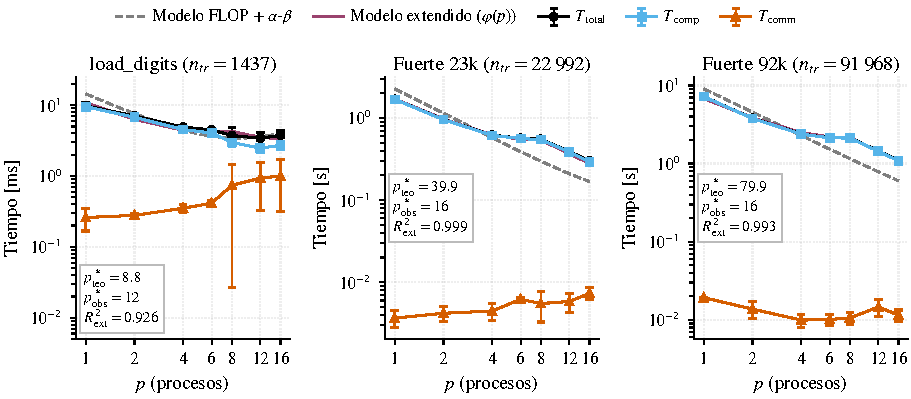
\includegraphics[width=0.66\textwidth]{tiempos_vs_p}
\begin{columns}[T]
\column{0.32\textwidth}\cifra{7.21 s $\to$ 1.09 s}{92k, de $p=1$ a $p=16$}
\column{0.32\textwidth}\cifra[exito]{$\le1.1$\,\% (92k)}{comunicación máxima: 1.06\,\% con $p=16$; $\le2.5$\,\% en 23k}
\column{0.32\textwidth}\cifra[alerta]{3\,\% $\to$ 27\,\%}{comunicación en \texttt{load\_digits}}
\end{columns}
\end{frame}

\begin{frame}{¿En qué se va el tiempo?}
\centering
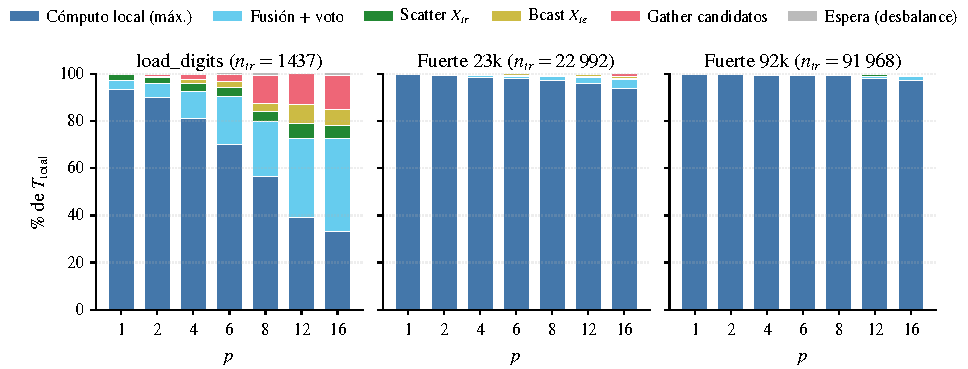
\includegraphics[width=0.84\textwidth]{desglose}
\begin{itemize}\small
\item En los conjuntos grandes domina el \textbf{cómputo local}: la comunicación es marginal.
\item En \texttt{load\_digits} ($\approx10$\,ms de trabajo), la fusión y las colectivas crecen con $p$ y el tiempo deja de bajar cerca de $p=8$--12.
\end{itemize}
\end{frame}

\begin{frame}{Colectivas: siguen U6.1, salvo el Scatter de 92k}
\centering
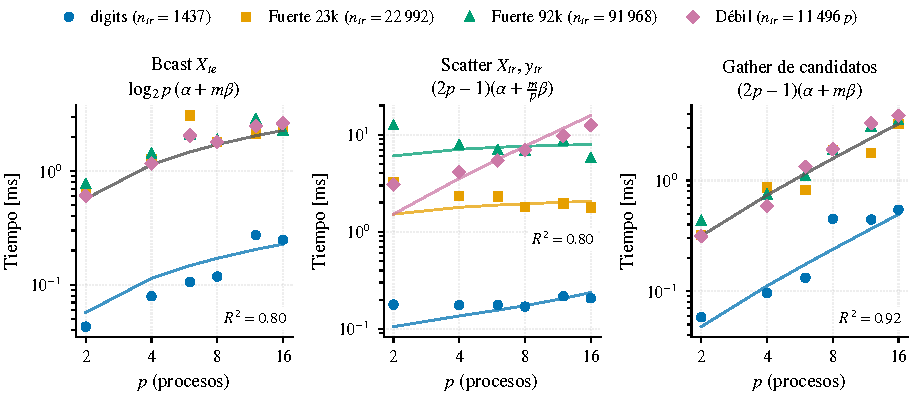
\includegraphics[width=0.78\textwidth]{validacion_colectivas}
\begin{columns}[T]
\column{0.32\textwidth}{\small\textbf{Bcast} $\propto\log_2p$: 0.77, 1.43 y 2.28\,ms con $p=2,4,16$ ($R^2=0.80$).}
\column{0.32\textwidth}{\small\textbf{Scatter}: crece con los bytes; débil de 3.1 a 12.5\,ms ($R^2=0.80$). En 92k baja (12.6$\to$5.7\,ms).}
\column{0.32\textwidth}{\small\textbf{Gather} $\propto(2p-1)$: de 0.43 a 3.52\,ms ($R^2=0.92$).}
\end{columns}
\end{frame}

\begin{frame}{Speedup y eficiencia (escalabilidad fuerte)}
\begin{columns}[c]
\column{0.68\textwidth}
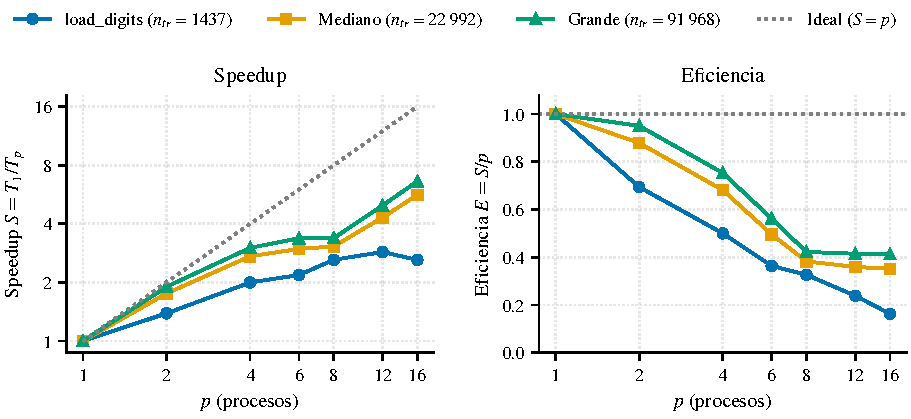
\includegraphics[width=\textwidth]{speedup_eficiencia}
\column{0.30\textwidth}
\cifra{$S=6.61$}{92k con $p=16$, $E=0.41$}
\cifra[acento]{$S=5.63$}{23k con $p=16$}
\cifra[alerta]{$S_{\text{máx}}=2.87$}{\texttt{load\_digits}, $p=12$}
{\scriptsize Hyper-threading ($p=32$): 1.208\,s, \textbf{peor} que 1.091\,s con 16 núcleos físicos.}
\end{columns}
\end{frame}

\begin{frame}{Normalización de la expresión teórica}
\begin{columns}[T]
\column{0.5\textwidth}
\begin{block}{Modelo (Big-O $\to$ constantes medidas)}
\[
T_p=\frac{A}{p}+Bp+C\log_2p+D
\]
{\small $A=c_1\ntr\nte d$; $B$, $C$, $D$ con $\alpha$ y $\beta$ de U6.1.}
\end{block}
\begin{block}{Procedimiento}
\begin{enumerate}\setlength{\itemsep}{1pt}\small
\item $c_1,c_2$: NNLS sobre $\tsub{comp}$.
\item $\alpha,\beta$: NNLS sobre $\tsub{comm}$ $\Rightarrow$ $\alpha=6.5\,\mu$s, $1/\beta=7.7$\,GB/s.
\item Se ajusta con las series fuertes; se valida dejando una serie fuera.
\end{enumerate}
\end{block}
\column{0.46\textwidth}
\begin{alertblock}{El modelo puro de FLOP no basta}
$R^2=0.29$, 0.61 y 0.77 (digits, 23k, 92k): sobrestima la ganancia del cómputo.
\end{alertblock}
\begin{exampleblock}{Con el factor medido $\varphi(p)$}
Sustituir $A/p$ por $A\,\varphi(p)/p$ eleva el ajuste a $R^2=0.926$, 0.999 y \textbf{0.993}.\\
{\small Ej.\ 92k, $p=8$: modelo 2.144\,s vs.\ medido 2.134\,s (0.5\,\%).}
\end{exampleblock}
\begin{block}{Fuera de muestra (no solo ajuste)}
\footnotesize Con dos series se predice la tercera: $R^2=0.998$ (23k), 0.994 (92k) y 0.66 en digits (dominan los overheads).
\end{block}
\end{columns}
\end{frame}

\begin{frame}{Cantidad óptima de procesos $p^*$}
\begin{columns}[T]
\column{0.5\textwidth}
\begin{block}{Derivada del modelo}
\[
\frac{\partial T_p}{\partial p}=-\frac{A}{p^2}+B+\frac{C}{p\ln2}=0\ \Rightarrow\ p^*\approx\sqrt{\frac{A}{B}}
\]
\end{block}
\vspace{6pt}
\small
\begin{tabular}{@{}lcc@{}}\toprule
Serie & $p^*$ teórico & Observado\\\midrule
\texttt{load\_digits} & 8.8 & meseta 8--16\\
Fuerte 23k & 39.9 & sigue bajando a 16\\
Fuerte 92k & 79.9 & sigue bajando a 16\\\bottomrule
\end{tabular}
\column{0.46\textwidth}
\begin{exampleblock}{Lectura}
\begin{itemize}\setlength{\itemsep}{2pt}
\item \textbf{digits}: $T(8)$, $T(12)$ y $T(16)$ coinciden dentro de $1\sigma$: concuerda con $p^*=8.8$.
\item \textbf{23k y 92k}: $p^*$ supera los 16 núcleos disponibles; el tiempo baja hasta $p=16$, pero con $E\approx0.35$--0.41.
\item \textbf{Con $\varphi(p)$}: mínimo en $p=16$ dentro del rango medido. Con $\varphi$ saturado (2.52): $p^*_{\mathrm{ext}}=17.2$, 89.9 y 180 (los dos últimos, extrapolación).
\end{itemize}
\end{exampleblock}
\end{columns}
\end{frame}

\begin{frame}{Rendimiento en FLOP/s}
\begin{columns}[c]
\column{0.58\textwidth}
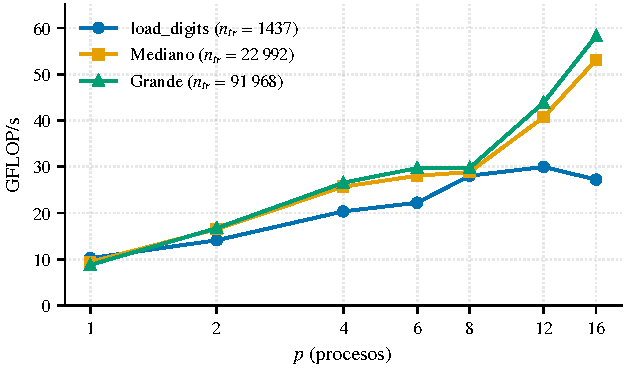
\includegraphics[width=\textwidth]{gflops_vs_p}
\column{0.40\textwidth}
\cifra{8.8 $\to$ 58.3 GFLOP/s}{equivalentes (FLOP del algoritmo); 92k, de $p=1$ a $p=16$}
\begin{block}{Coherente con la teoría (U2.1)}
Con $p=1$ medimos 8.8--9.4 GFLOP/s por núcleo, dentro del rango de 4--12 GFLOP/s por núcleo del curso.
\end{block}
{\small FLOP $=3d\,\ntr\nte$: la región paralelizable (el ``entrenamiento'' del enunciado) son las distancias contra $X_{tr}$; todas las operaciones cuentan igual (U6.2).}
\end{columns}
\end{frame}

% =====================================================================
\parte{4}{¿Por qué se satura?}{Contención intra-nodo, métricas de escalabilidad y comparación de descomposiciones}

\begin{frame}{El límite es la contención intra-nodo, no MPI}
\begin{columns}[c]
\column{0.56\textwidth}
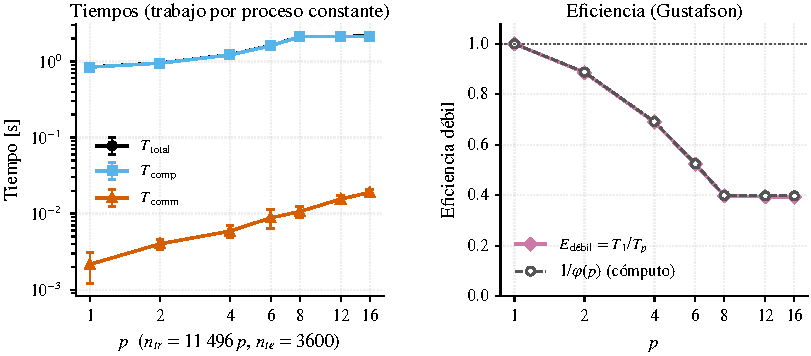
\includegraphics[width=\textwidth]{escalabilidad_debil}
\column{0.42\textwidth}
\begin{block}{Serie débil: mismo trabajo por proceso}
\[
\varphi(p)=\frac{\tsub{comp}(p)}{\tsub{comp}(1)}:\ 1.00\to\mathbf{2.52}
\]
mientras $\tsub{comm}\le0.019$\,s.
\end{block}
\begin{alertblock}{Diagnóstico sin comunicación (job 64273)}
Con 16 procesos, el GEMM tarda $\mathbf{2.12\times}$ más y el top-$k$ $1.76\times$ más.
\end{alertblock}
\begin{block}{Causas posibles (U6.4)}Potencia $\propto f^3$ y ``la memoria es el mayor cuello de botella''. Sin contadores de hardware no separamos cuál domina.\end{block}
\end{columns}
\end{frame}

\begin{frame}{Métricas de escalabilidad del curso (U2.1, U6.2)}
\begin{columns}[T]
\column{0.55\textwidth}
\scriptsize
\begin{tabular}{@{}rrrrrr@{}}\toprule
$p$ & $T_p$ [s] & $S$ & $E$ & $T_0/W$ & $CE/CE_1$\\\midrule
1 & 7.208 & 1.00 & 1.00 & 0.00 & 1.00\\
2 & 3.793 & 1.90 & 0.95 & 0.05 & 1.05\\
4 & 2.394 & 3.01 & 0.75 & 0.33 & 1.33\\
8 & 2.134 & 3.38 & 0.42 & 1.37 & 2.37\\
16 & 1.091 & 6.61 & 0.41 & 1.42 & 2.42\\\bottomrule
\end{tabular}\\[2pt]
{\scriptsize Fuerte 92k.}
\column{0.42\textwidth}
\begin{itemize}\small\setlength{\itemsep}{2pt}
\item \textbf{Consistencia:} $E=1/(1+T_0/W)=1/(1+1.42)=0.413$ \checkmark
\item \textbf{Amdahl:} $f_s$ varía entre 0.05 y 0.20: no hay fracción serial fija.
\item \textbf{Gustafson (empírico):} $S_G=p\,E_{\text{débil}}=6.28$ con $p=16$ (serie débil; con esta tabla, $pE=S$).
\item \textbf{Energía:} $2.42\times$ la de $p=1$ para ir $6.6\times$ más rápido.
\end{itemize}
\end{columns}
\vspace{4pt}
\begin{exampleblock}{Escalable algorítmicamente, limitado experimentalmente}
Isoeficiencia: $\ntr=\Omega(p^2/d)$ y $\nte=\Omega(p)$; tiempo lineal con el trabajo (pendientes 1.05, 0.98 y 0.95). En Khipu, $E_{\text{débil}}(16)=0.39$ por $\varphi$.
\end{exampleblock}
\end{frame}

\begin{frame}{Dos descomposiciones: DAG vs.\ réplica de $X_{tr}$}
\begin{columns}[c]
\column{0.6\textwidth}
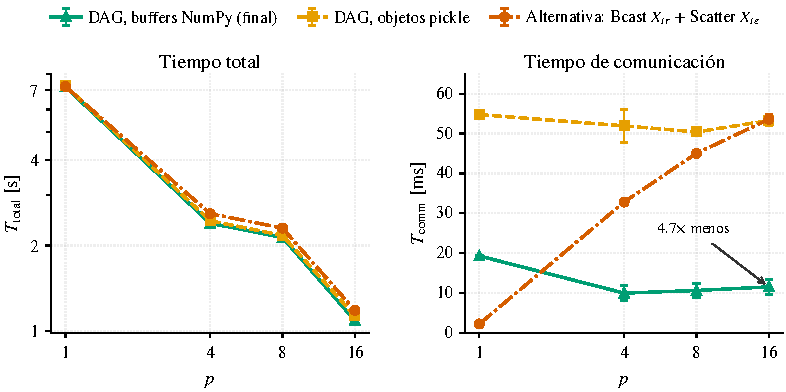
\includegraphics[width=\textwidth]{comparacion_variantes}
\column{0.38\textwidth}
\begin{block}{Teoría (Alg.\ 6)}
\[
T^{\mathrm{rep}}_{\mathrm{bc}}\approx\log_2p\;8\ntr(d+1)\beta
\]
Difunde 47.8\,MB en vez de 1.8\,MB; requiere $\nte=\Omega(p\log p)$.
\end{block}
\cifra[exito]{$4.7\times$ menos}{comunicación del DAG con $p=16$: 11.5 vs.\ 53.6\,ms}
{\scriptsize El modelo acierta la forma (Bcast $\ge97$\,\% de $\tsub{comm}$), pero subestima la magnitud 2.1--2.6$\times$.}
\end{columns}
\end{frame}

\begin{frame}{Mejoras propuestas}
\begin{columns}[T]
\column{0.5\textwidth}
\begin{block}{Contra la contención (el límite real)}
\begin{itemize}\setlength{\itemsep}{1pt}\small
\item Más nodos con menos procesos por nodo.
\item \texttt{float32} (exacto: $d\cdot256<2^{24}$) y bloques que quepan en caché.
\item Fusionar distancias y selección sin materializar la matriz.
\end{itemize}
\end{block}
\column{0.46\textwidth}
\begin{block}{Con la teoría del curso}
\begin{itemize}\setlength{\itemsep}{1pt}\small
\item Reducción en árbol del top-$k$ (U6.1): $\log p(\alpha+3k\nte\beta)$.
\item No bloqueante (U3.3): ganancia acotada por $\tsub{comm}/\tsub{total}$.
\item Híbrido MPI+OpenMP (U4.5).
\item GPU (U6.4) y particionamiento 2D (U6.3).
\end{itemize}
\end{block}
\end{columns}
\end{frame}

\begin{frame}{Conclusiones}
\begin{columns}[T]
\column{0.5\textwidth}
\begin{exampleblock}{1. Correcto}
El KNN según el DAG reproduce \textbf{exactamente} al secuencial para todo $p$ (129/129).
\end{exampleblock}
\begin{exampleblock}{2. Algorítmicamente escalable}
Comunicación $\le1.1$\,\% (92k); colectivas en general según U6.1, salvo el Scatter de 92k. Experimentalmente limitado en un nodo: $E_{\text{débil}}(16)=0.39$.
\end{exampleblock}
\column{0.46\textwidth}
\begin{block}{3. Rendimiento}
$S=6.61$ y 58.3\,GFLOP/s equivalentes con 16 núcleos.
\end{block}
\begin{alertblock}{4. Teoría vs.\ experimento}
La brecha frente al ideal se explica con $\varphi(p)$ medido: el modelo normalizado se ajusta con error de 1.8--2.8\,\% y predice fuera de muestra con 1.8--3.6\,\%.
\end{alertblock}
\end{columns}
\end{frame}

\begin{frame}{Fuentes}
\begin{columns}[T]
\column{0.5\textwidth}
\begin{block}{Base teórica}
\footnotesize J.~Fiestas, U1--U6 (Foster/Flynn, DAG, PRAM, MPI, Broadcast, escalabilidad, matrices, CUDA), CS4052, UTEC, 2026.\\
J.~JáJá (1992); R.~P.~Brent (1974); I.~Foster (1995).
\end{block}
\begin{block}{KNN y colectivas}
\footnotesize Fix y Hodges (1951); Cover y Hart (1967); Thakur, Rabenseifner y Gropp (2005); Aparício et al.\ (2007); Patwary et al.\ (2016).
\end{block}
\begin{block}{Software y datos}
\footnotesize mpi4py, NumPy, scikit-learn (\texttt{load\_digits}), documentación de Khipu.
\end{block}
\column{0.46\textwidth}
\begin{block}{Uso de IA (Claude, vía Claude Code)}
\scriptsize
\renewcommand{\arraystretch}{1.25}
\begin{tabular}{@{}>{\raggedright\arraybackslash}p{0.33\linewidth}>{\raggedright\arraybackslash}p{0.61\linewidth}@{}}
\textbf{Ámbito} & \textbf{Control y verificación}\\\midrule
Revisión analítica & derivaciones verificadas a mano con U2.2, U6.1 y U6.2\\
Búsqueda bibliográfica & cada referencia comprobada en su repositorio oficial\\
Estructuración en \LaTeX & compilación y revisión por los autores\\
Coherencia y cálculos & cifras regeneradas desde los CSV; 129/129 pruebas\\
\end{tabular}\\[3pt]
\textbf{Impacto:} agilizó la revisión, las referencias y la maquetación; las mediciones son 100\,\% de Khipu y el análisis es del equipo.
\end{block}
\end{columns}
\end{frame}

{\setbeamertemplate{footline}{}
\begin{frame}[plain]
\centering
\vspace{1.6cm}
{\color{navy}\fontsize{20}{24}\selectfont\bfseries ¡Muchas gracias por su atención!}\\[8pt]
{\color{cian}\rule{2.6cm}{1.6pt}}\\[10pt]
{\color{navy}\small\bfseries Paralelización del clasificador KNN con MPI}\\[8pt]
{\color{gristxt}\scriptsize Juan David Velo Poma \quad$\cdot$\quad Farid Jack Aquino Castro \quad$\cdot$\quad Josue Nehemias Velo Poma}\\[4pt]
{\color{gristxt}\scriptsize Universidad de Ingeniería y Tecnología (UTEC) -- 2026}\\[10pt]
{\color{cian}\scriptsize Código y resultados: \texttt{github.com/Juan-Velo/cpd\_proyecto\_final}}
\end{frame}}

% =====================================================================
\appendix
\parte{A}{Anexo}{Diapositivas de respaldo para la ronda de preguntas}

\begin{frame}{Anexo: escalabilidad fuerte completa}
\centering\scriptsize
\setlength{\tabcolsep}{3.5pt}
\begin{tabular}{@{}r|rrrr|rrrr|rrrr@{}}\toprule
& \multicolumn{4}{c|}{digits} & \multicolumn{4}{c|}{Fuerte 23k} & \multicolumn{4}{c}{Fuerte 92k}\\
$p$ & $T_p$ [ms] & $\tsub{comm}$ [ms] & $S$ & $E$ & $T_p$ [s] & $\tsub{comm}$ [ms] & $S$ & $E$ & $T_p$ [s] & $\tsub{comm}$ [ms] & $S$ & $E$\\\midrule
1 & 9.75 & 0.26 & 1.00 & 1.00 & 1.684 & 3.7 & 1.00 & 1.00 & 7.208 & 19.3 & 1.00 & 1.00\\
2 & 7.02 & 0.27 & 1.39 & 0.69 & 0.958 & 4.2 & 1.76 & 0.88 & 3.793 & 13.7 & 1.90 & 0.95\\
4 & 4.88 & 0.35 & 2.00 & 0.50 & 0.618 & 4.5 & 2.72 & 0.68 & 2.394 & 9.9 & 3.01 & 0.75\\
6 & 4.47 & 0.42 & 2.18 & 0.36 & 0.566 & 6.2 & 2.97 & 0.50 & 2.139 & 10.1 & 3.37 & 0.56\\
8 & 3.73 & 0.74 & 2.61 & 0.33 & 0.550 & 5.5 & 3.06 & 0.38 & 2.134 & 10.6 & 3.38 & 0.42\\
12 & 3.40 & 0.93 & 2.87 & 0.24 & 0.390 & 5.8 & 4.31 & 0.36 & 1.449 & 14.6 & 4.98 & 0.41\\
16 & 3.74 & 1.00 & 2.61 & 0.16 & 0.299 & 7.3 & 5.63 & 0.35 & 1.091 & 11.5 & 6.61 & 0.41\\\bottomrule
\end{tabular}
\end{frame}

\begin{frame}{Anexo: comunicación con las fórmulas de U6.1}
\begin{columns}[T]
\column{0.5\textwidth}
\begin{block}{DAG (Alg.\ 5), $m$ en bytes}
\vspace{-6pt}
\begin{align*}
\tsub{sc}&=2(2p-1)\alpha+\tfrac{2p-1}{p}\,8\ntr(d+1)\beta\\
\tsub{bc}&=\log_2p\,(\alpha+8\nte d\beta)\\
\tsub{ga}&=(2p-1)(\alpha+24k\nte\beta)
\end{align*}
\end{block}
\column{0.46\textwidth}
\begin{block}{Eficiencia (análoga a U6.3)}
\[
\begin{aligned}
E&=O\!\left(\big[1+\varepsilon\big]^{-1}\right),\\
\varepsilon&=\tfrac{p\log p}{\nte d\ntr}+\tfrac{p\log p}{\ntr}+\tfrac{p}{\nte}+\tfrac{p^2k}{\ntr d}
\end{aligned}
\]
{\scriptsize Bcast de $X_{te}$ (como en U6.3) + Scatter de $X_{tr}$ ($p/\nte$) + Gather y fusión ($p^2k/\ntr d$).}
\end{block}
\begin{block}{Overhead e isoeficiencia (U6.2)}
$T_0\approx Bp^2+Cp\log p+Dp$ $\Rightarrow$ $\ntr=\Omega(p^2/d)$, $\nte=\Omega(p)$.
\end{block}
\end{columns}
\end{frame}

\begin{frame}{Anexo: variante alternativa {\normalsize\mdseries\color{gristxt}(Alg.~6 del informe)}}
\begin{columns}[T]
\column{0.6\textwidth}
\setcounter{algocf}{5}
\begin{algorithm}[H]
\caption{Variante alternativa: réplica de $X_{tr}$ y reparto de $X_{te}$ ($p$ procesos, rango $r$)}\label{alg:rep}
\KwIn{$X_{tr},y_{tr},X_{te}$ en $P_0$; $k$; $p$}
\KwOut{$\hat y$ y exactitud en $P_0$}
$m_r\leftarrow\lfloor\nte/p\rfloor+[\,r<\nte\bmod p\,]$ \tcp*{bloques de consultas}
$(X_{tr},y_{tr})\leftarrow\textsc{Bcast}((X_{tr},y_{tr}),0)$ \tcp*{\texttt{comm.bcast} / \texttt{Bcast}}
$(X_{te}^{(r)})_{r=0}^{p-1}\leftarrow\textsc{Scatter}(X_{te},0)$ \tcp*{\texttt{comm.scatter} / \texttt{Scatterv}}
\ForAllPar{$r\leftarrow0$ \KwTo $p-1$}{
  \For{$j\leftarrow1$ \KwTo $m_r$}{
    $N_j\leftarrow$ $k$ mínimos de $\textsc{Distancia}(X^{(r)}_{te}[j],X_{tr}[\cdot])$ \tcp*{\texttt{argpartition}, $O(\ntr)$}
    $\hat y^{(r)}[j]\leftarrow$ mayoría de $y_{tr}[N_j]$\;
  }
}
$\hat y\leftarrow\textsc{Gather}(\hat y^{(r)},0)$ \tcp*{\texttt{comm.gather} / \texttt{Gatherv}}
\lIf{$r=0$}{exactitud $\leftarrow\frac1{\nte}\sum_j[\hat y[j]=y_{te}[j]]$}
\end{algorithm}
\column{0.38\textwidth}
\begin{block}{Medido vs.\ predicho (Bcast de $X_{tr}$)}
\small
\begin{tabular}{@{}rrr@{}}\toprule
$p$ & medido & predicho\\\midrule
4 & 32.0\,ms & 12.5\,ms\\
8 & 44.4\,ms & 18.7\,ms\\
16 & 52.7\,ms & 25.0\,ms\\\bottomrule
\end{tabular}
\end{block}
{\small Con $\beta$ ajustado en las series del DAG.}
\end{columns}
\end{frame}

\begin{frame}{Anexo: exactitud y escalabilidad con el tamaño}
\begin{columns}[c]
\column{0.55\textwidth}
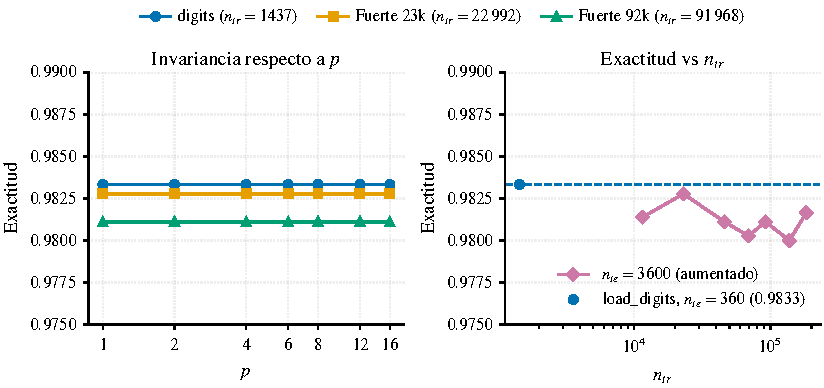
\includegraphics[width=\textwidth]{accuracy}\\
{\scriptsize Exactitud idéntica para todo $p$; 0.9800--0.9828 con datos aumentados.}
\column{0.43\textwidth}
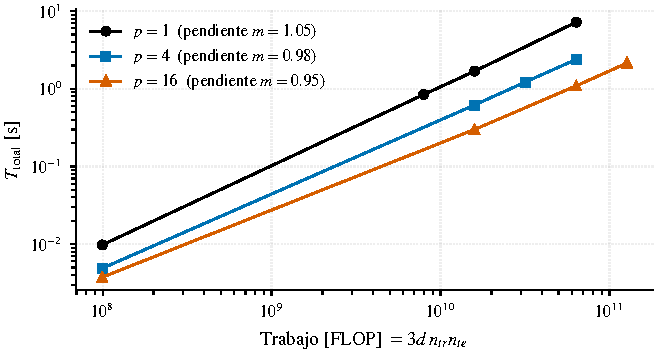
\includegraphics[width=\textwidth]{tiempo_vs_N}\\
{\scriptsize Tiempo lineal con el trabajo: pendientes 1.05, 0.98 y 0.95.}
\end{columns}
\end{frame}

\end{document}
